%=====================================================================
%==========================PAQUETES y DEFICION DEL ARCHIVO============
\documentclass[12pt]{article}
\usepackage[spanish,mexico]{babel}
	\selectlanguage{spanish}
\usepackage{graphicx}
\usepackage{amsmath}
\usepackage{wrapfig}
\usepackage{float}
\usepackage[utf8]{inputenc}
\usepackage[utf8]{inputenc}
\usepackage{color}
\usepackage{graphicx}
\graphicspath{{images/}}

\setlength{\parskip}{\medskipamount}
\setlength{\parindent}{0pt}
\definecolor{labelcolor}{RGB}{100,0,0}


\usepackage{vmargin}
\setmarginsrb{3 cm}{1.0 cm}{3 cm}{1.0 cm}{1 cm}{1.5 cm}{1 cm}{1.5 cm}
\usepackage{listings}
%=====================================================================
%=======================DATOS AUTOR===================================
%=====================================================================
\title{Actividad 8: Iniciandose en Computo Simbolico con Maxima}
\author{Martin Alejandro Paredes Sosa}
\date{Abril, 2016}
%=====================================================================
%=====================================================================
\begin{document}
\maketitle
%====================================================
%====================================================

\section{Introducción}


%====================================================
%====================================================

\section{Geometria en tres dimensiones}
Esta sección consta en enseñarnos herramientas para geometria tridimensional.
%====================================================
\subsection{Vectores y Algebra lineal}
En maxima hay forma de realizar operaciones con vectores, como es el producto punto y el producto cruz.

\noindent

\begin{minipage}[t]{8ex}{\color{red}\bf
\begin{verbatim}
(%i1) 
\end{verbatim}}
\end{minipage}
\begin{minipage}[t]{\textwidth}{\color{blue}
\begin{verbatim}
a: [6,2,5];
b: [8,-3,0];
a.b;
load(vect);
express(a~b);
c: [-5,2,9];
express(a.(b~c));
\end{verbatim}}
\end{minipage}

\begin{math}\displaystyle
\parbox{8ex}{\color{labelcolor}(\%o1) }
[6,2,5]
\end{math}

\begin{math}\displaystyle
\parbox{8ex}{\color{labelcolor}(\%o2) }
[8,−3,0]
\end{math}

\begin{math}\displaystyle
\parbox{8ex}{\color{labelcolor}(\%o3) }
42
\end{math}

\begin{math}\displaystyle
\parbox{8ex}{\color{labelcolor}(\%o4) }
/usr/share/maxima/5.34.1/share/vector/vect.mac
\end{math}

\begin{math}\displaystyle
\parbox{8ex}{\color{labelcolor}(\%o5) }
[15,40,−34]
\end{math}

\begin{math}\displaystyle
\parbox{8ex}{\color{labelcolor}(\%o6) }
[−5,2,9]
\end{math}

\begin{math}\displaystyle
\parbox{8ex}{\color{labelcolor}(\%o7) }
−301
\end{math}

%====================================================
%====================================================
\subsection{Lineas, Planos y Superficies Cuadraticas}
Con maxima se pueden definir ecuaciones de planos y superficies, con el objetivo de poder visualizarlos.
\begin{minipage}[t]{8ex}{\color{red}\bf
\begin{verbatim}
(%i1) 
\end{verbatim}}
\end{minipage}
\begin{minipage}[t]{\textwidth}{\color{blue}
\begin{verbatim}
load(draw);
ellips1: x^2/3+0.5*x*y+z   = 0;
draw3d(enhanced3d = true,
       palette = [cyan,blue,cyan],
       implicit(ellips1, x,-100,100, y,-100,100, z,-100,100));
\end{verbatim}}
\end{minipage}

\begin{math}\displaystyle
\parbox{8ex}{\color{labelcolor}(\%o1) }
/usr/share/maxima/5.34.1/share/draw/draw.lisp
\end{math}

\begin{math}\displaystyle
\parbox{8ex}{\color{labelcolor}(\%o2) }
z+0.5\,x\,y+\frac{{x}^{2}}{3}=0
\end{math}

\begin{math}\displaystyle
\parbox{8ex}{\color{labelcolor}(\%o3) }
[\mathrm{gr3d}\left( implicit\right) ]
\end{math}
\begin{figure}[H]
\centering
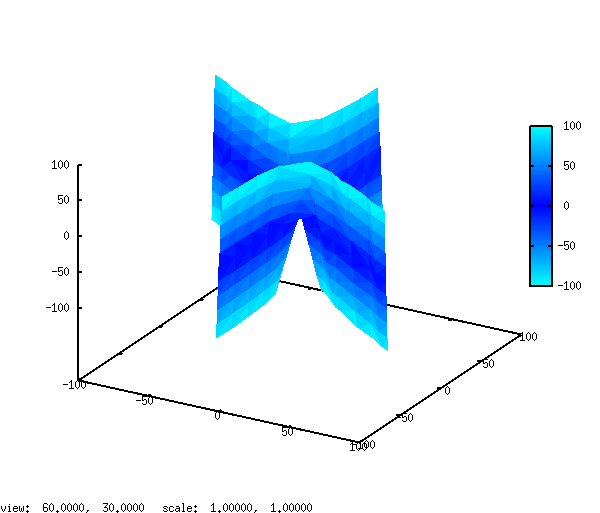
\includegraphics[scale=0.5]{1.png}
\caption{Grafica de la superficie $z+0.5\,x\,y+\frac{{x}^{2}}{3}=0$}
\end{figure}
%====================================================
%====================================================
\subsection{Funciones Vectoriales}
Maxima nos permite trabajar con funciones vectoriales como graficar, parametrizar y realizar operaciones con ellas.

\noindent
\begin{minipage}[t]{8ex}{\color{red}\bf
\begin{verbatim}
(%i1) 
\end{verbatim}}
\end{minipage}
\begin{minipage}[t]{\textwidth}{\color{blue}
\begin{verbatim}
load(draw);
load(eigen);
load(vect);
draw3d(parametric(cos(t),cos(4*t),-sin(t),t, -4,4));
r(t) := [cos(t), sin(t), t];
float(r(1));
limit(r(t),t,2);
limit(r(t),t, 2, plus);
limit(r(t), t,3,minus);
define(rp(t), diff(r(t),t));
float(rp(1));
define( T(t), trigsimp( uvect( rp(t) ) ) );
define(Tp(t), diff( T(t), t));
define( N(t), trigsimp( uvect( Tp(t) ) ) );
express(T(t)~N(t));
define(B(t),trigsimp(%));
float(B(1));
\end{verbatim}}
\end{minipage}
%%% OUTPUT:
\begin{math}\displaystyle
\parbox{8ex}{\color{labelcolor}(\%o1) }
/usr/share/maxima/5.34.1/share/draw/draw.lisp
\end{math}

\begin{math}\displaystyle
\parbox{8ex}{\color{labelcolor}(\%o2) }
/usr/share/maxima/5.34.1/share/matrix/eigen.mac
\end{math}

\begin{math}\displaystyle
\parbox{8ex}{\color{labelcolor}(\%o3) }
/usr/share/maxima/5.34.1/share/vector/vect.mac
\end{math}

\begin{math}\displaystyle
\parbox{8ex}{\color{labelcolor}(\%o4) }
[\mathrm{gr3d}\left( parametric\right) ]
\end{math}

\begin{figure}[H]
\centering
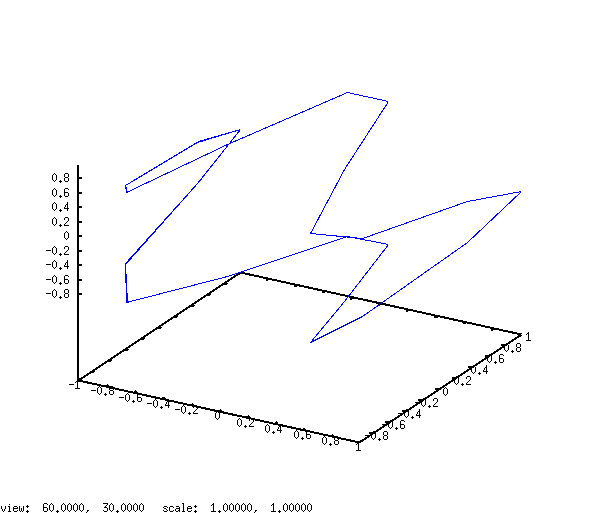
\includegraphics[scale=0.5]{2.png}
\caption{Trayectoria descrita por $(cos(t),cos(4*t),-sin(t))$ donde $t\in[-4,4]$ }
\end{figure}

\begin{math}\displaystyle
\parbox{8ex}{\color{labelcolor}(\%o5) }
\mathrm{r}\left( t\right) :=[\mathrm{cos}\left( t\right) ,\mathrm{sin}\left( t\right) ,t]
\end{math}

\begin{math}\displaystyle
\parbox{8ex}{\color{labelcolor}(\%o6) }
[0.5403023058681398,0.8414709848078965,1.0]
\end{math}

\begin{math}\displaystyle
\parbox{8ex}{\color{labelcolor}(\%o7) }
[\mathrm{cos}\left( 2\right) ,\mathrm{sin}\left( 2\right) ,2]
\end{math}

\begin{math}\displaystyle
\parbox{8ex}{\color{labelcolor}(\%o8) }
[\mathrm{cos}\left( 2\right) ,\mathrm{sin}\left( 2\right) ,2]
\end{math}

\begin{math}\displaystyle
\parbox{8ex}{\color{labelcolor}(\%o9) }
[\mathrm{cos}\left( 3\right) ,\mathrm{sin}\left( 3\right) ,3]
\end{math}

\begin{math}\displaystyle
\parbox{8ex}{\color{labelcolor}(\%o10) }
\mathrm{rp}\left( t\right) :=[−\mathrm{sin}\left( t\right) ,\mathrm{cos}\left( t\right) ,1]
\end{math}

\begin{math}\displaystyle
\parbox{8ex}{\color{labelcolor}(\%o11) }
[−0.8414709848078965,0.5403023058681398,1.0]
\end{math}

\begin{math}\displaystyle
\parbox{8ex}{\color{labelcolor}(\%o12) }
\mathrm{T}\left( t\right) :=[−\frac{\mathrm{sin}\left( t\right) }{\sqrt{2}},\frac{\mathrm{cos}\left( t\right) }{\sqrt{2}},\frac{1}{\sqrt{2}}]
\end{math}

\begin{math}\displaystyle
\parbox{8ex}{\color{labelcolor}(\%o13) }
\mathrm{Tp}\left( t\right) :=[−\frac{\mathrm{cos}\left( t\right) }{\sqrt{2}},−\frac{\mathrm{sin}\left( t\right) }{\sqrt{2}},0]
\end{math}

\begin{math}\displaystyle
\parbox{8ex}{\color{labelcolor}(\%o14) }
\mathrm{N}\left( t\right) :=[−\mathrm{cos}\left( t\right) ,−\mathrm{sin}\left( t\right) ,0]
\end{math}

\begin{math}\displaystyle
\parbox{8ex}{\color{labelcolor}(\%o15) }
[\frac{\mathrm{sin}\left( t\right) }{\sqrt{2}},−\frac{\mathrm{cos}\left( t\right) }{\sqrt{2}},\frac{{\mathrm{sin}\left( t\right) }^{2}}{\sqrt{2}}+\frac{{\mathrm{cos}\left( t\right) }^{2}}{\sqrt{2}}]
\end{math}

\begin{math}\displaystyle
\parbox{8ex}{\color{labelcolor}(\%o16) }
\mathrm{B}\left( t\right) :=[\frac{\mathrm{sin}\left( t\right) }{\sqrt{2}},−\frac{\mathrm{cos}\left( t\right) }{\sqrt{2}},\frac{1}{\sqrt{2}}]
\end{math}

\begin{math}\displaystyle
\parbox{8ex}{\color{labelcolor}(\%o17) }
[0.5950098395293859,−0.3820514243700897,0.7071067811865475]
\end{math}


\subsection{Longitud de Arco y Curvatura}
En maxima nos permite realizar las operaciones para calcular estas cualidades de ecuaciones paramétricas.

\noindent

\begin{minipage}[t]{8ex}{\color{red}\bf
\begin{verbatim}
(%i1) 
\end{verbatim}}
\end{minipage}
\begin{minipage}[t]{\textwidth}{\color{blue}
\begin{verbatim}
r(t) := [t, cos(t), sin(t)];
rp(t) := [1,-sin(t), cos(t)];
Tp(t) := [0,-cos(t), sin(t)]/sqrt(2);
sqrt(Tp(t) . Tp(t))/sqrt(rp(t).rp(t));
trigsimp(%);
define(kappa(t),%);
integrate(r(t),t);
g(t) := [2*t,3*sin(t),3*cos(t)];
define(gp(t) , diff(g(t),t));
integrate(trigsimp(sqrt(gp(t).gp(t))),t,0,2*%pi);
romberg(sqrt(gp(t).gp(t)),t,0,2*%pi);
\end{verbatim}}
\end{minipage}
%%% OUTPUT:
\begin{math}\displaystyle
\parbox{8ex}{\color{labelcolor}(\%o1) }
\mathrm{r}\left( t\right) :=[t,\mathrm{cos}\left( t\right) ,\mathrm{sin}\left( t\right) ]
\end{math}

\begin{math}\displaystyle
\parbox{8ex}{\color{labelcolor}(\%o2) }
\mathrm{rp}\left( t\right) :=[1,−\mathrm{sin}\left( t\right) ,\mathrm{cos}\left( t\right) ]
\end{math}

\begin{math}\displaystyle
\parbox{8ex}{\color{labelcolor}(\%o3) }
\mathrm{Tp}\left( t\right) :=\frac{[0,−\mathrm{cos}\left( t\right) ,\mathrm{sin}\left( t\right) ]}{\sqrt{2}}
\end{math}

\begin{math}\displaystyle
\parbox{8ex}{\color{labelcolor}(\%o4) }
\frac{\sqrt{\frac{{\mathrm{sin}\left( t\right) }^{2}}{2}+\frac{{\mathrm{cos}\left( t\right) }^{2}}{2}}}{\sqrt{{\mathrm{sin}\left( t\right) }^{2}+{\mathrm{cos}\left( t\right) }^{2}+1}}
\end{math}

\begin{math}\displaystyle
\parbox{8ex}{\color{labelcolor}(\%o5) }
\frac{1}{2}
\end{math}

\begin{math}\displaystyle
\parbox{8ex}{\color{labelcolor}(\%o6) }
\kappa\left( t\right) :=\frac{1}{2}
\end{math}

\begin{math}\displaystyle
\parbox{8ex}{\color{labelcolor}(\%o7) }
[\frac{{t}^{2}}{2},\mathrm{sin}\left( t\right) ,−\mathrm{cos}\left( t\right) ]
\end{math}

\begin{math}\displaystyle
\parbox{8ex}{\color{labelcolor}(\%o8) }
\mathrm{g}\left( t\right) :=[2\,t,3\,\mathrm{sin}\left( t\right) ,3\,\mathrm{cos}\left( t\right) ]
\end{math}

\begin{math}\displaystyle
\parbox{8ex}{\color{labelcolor}(\%o9) }
\mathrm{gp}\left( t\right) :=[2,3\,\mathrm{cos}\left( t\right) ,−3\,\mathrm{sin}\left( t\right) ]
\end{math}

\begin{math}\displaystyle
\parbox{8ex}{\color{labelcolor}(\%o10) }
2\,\sqrt{13}\,\pi 
\end{math}

\begin{math}\displaystyle
\parbox{8ex}{\color{labelcolor}(\%o11) }
22.65434679827795
\end{math}
%===================================================================
%===================================================================
\section{Funciones de varias varibles}
Maxima tiene la habilidad de trabajar con funciones de varias varibles, así como graficarlas.
\noindent
\begin{minipage}[t]{8ex}{\color{red}\bf
\begin{verbatim}
(%i1) 
\end{verbatim}}
\end{minipage}
\begin{minipage}[t]{\textwidth}{\color{blue}
\begin{verbatim}
load(draw);
f(x,y) := (5*x^2-2*y^2)^0.25;
draw3d(explicit(f(x,y),x,-5,5,y,-5,5));
\end{verbatim}}
\end{minipage}

\begin{math}\displaystyle
\parbox{8ex}{\color{labelcolor}(\%o1) }
/usr/share/maxima/5.34.1/share/draw/draw.lisp
\end{math}

\begin{math}\displaystyle
\parbox{8ex}{\color{labelcolor}(\%o2) }
\mathrm{f}\left( x,y\right) :={\left( 5\,{x}^{2}−2\,{y}^{2}\right) }^{0.25}
\end{math}

\begin{math}\displaystyle
\parbox{8ex}{\color{labelcolor}(\%o3) }
[\mathrm{gr3d}\left( explicit\right) ]
\end{math}

\begin{figure}[H]
\centering
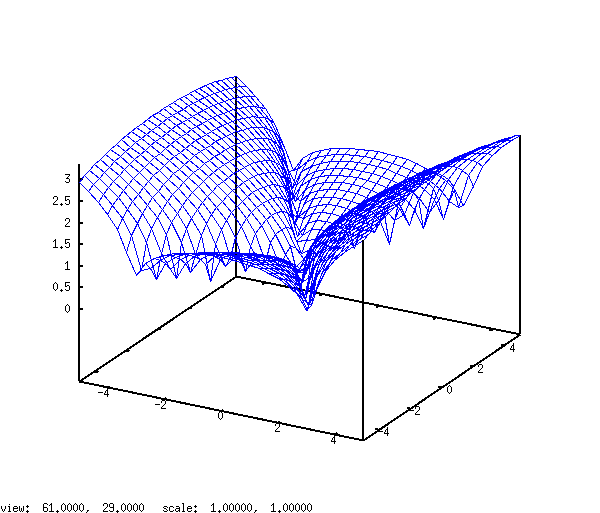
\includegraphics[scale=0.5]{3.png}
\caption{Superficie $f(x,y)= (5*x^2-2*y^2)^0.25$ }
\end{figure}

\noindent

\begin{minipage}[t]{8ex}{\color{red}\bf
\begin{verbatim}
(%i4) 
\end{verbatim}}
\end{minipage}
\begin{minipage}[t]{\textwidth}{\color{blue}
\begin{verbatim}
draw3d(enhanced3d = true,
       explicit(f(x,y),x,-5,5,y,-5,5),
       palette = [green,blue,cyan,red]);
\end{verbatim}}
\end{minipage}
:
\begin{math}\displaystyle
\parbox{8ex}{\color{labelcolor}(\%o4) }
[\mathrm{gr3d}\left( explicit\right) ]
\end{math}

\begin{figure}[H]
\centering
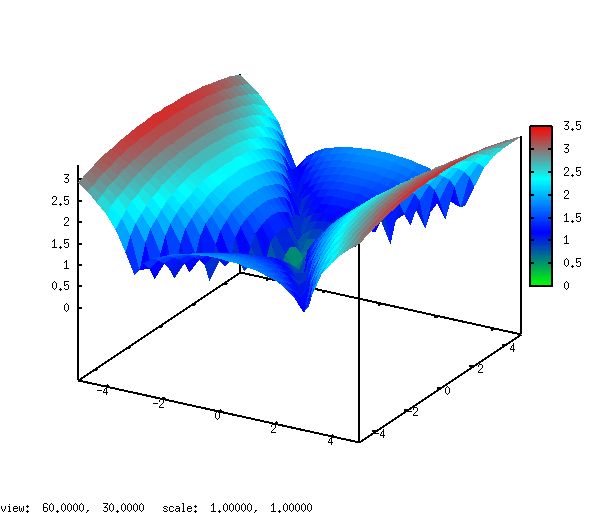
\includegraphics[scale=0.5]{4.png}
\caption{Superficie $f(x,y)= (5*x^2-2*y^2)^0.25$ }
\end{figure}

\noindent

\begin{minipage}[t]{8ex}{\color{red}\bf
\begin{verbatim}
(%i5) 
\end{verbatim}}
\end{minipage}
\begin{minipage}[t]{\textwidth}{\color{blue}
\begin{verbatim}
draw3d(explicit(f(x,y),x,-5,5,y,-5,5),
    contour_levels = 20,
    contour        = map);
\end{verbatim}}
\end{minipage}

\begin{math}\displaystyle
\parbox{8ex}{\color{labelcolor}(\%o5) }
[\mathrm{gr3d}\left( explicit\right) ]
\end{math}

\begin{figure}[H]
\centering
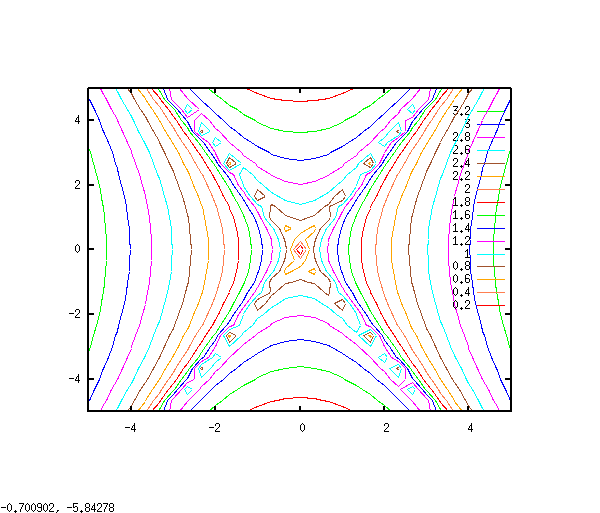
\includegraphics[scale=0.5]{5.png}
\caption{curvas de nivel de $f(x,y)= (5*x^2-2*y^2)^0.25$ }
\end{figure}

\noindent
\begin{minipage}[t]{8ex}{\color{red}\bf
\begin{verbatim}
(%i6) 
\end{verbatim}}
\end{minipage}
\begin{minipage}[t]{\textwidth}{\color{blue}
\begin{verbatim}
draw3d(enhanced3d = true,
       explicit(f(x,y),x,-5,5,y,-5,5),
       contour_levels = 20,
       contour = surface,
       palette = [green,blue,cyan,red],
       surface_hide = true);
\end{verbatim}}
\end{minipage}

\begin{math}\displaystyle
\parbox{8ex}{\color{labelcolor}(\%o6) }
[\mathrm{gr3d}\left( explicit\right) ]
\end{math}
\begin{figure}[H]
\centering
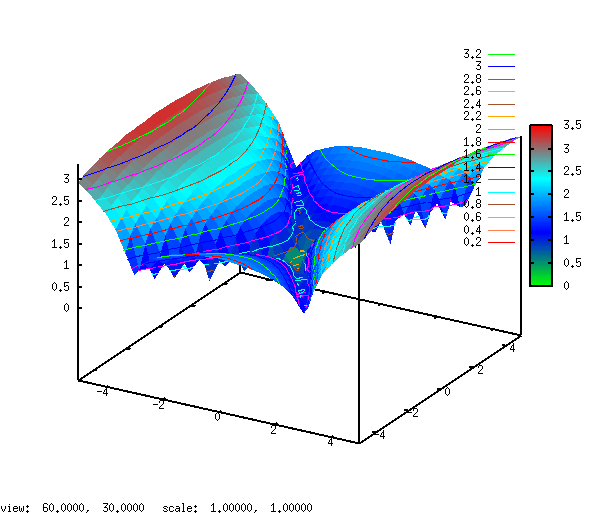
\includegraphics[scale=0.5]{6.png}
\caption{Superficie $f(x,y)= (5*x^2-2*y^2)^0.25$ }
\end{figure}


\end{document}

